\section{Related Work}
\label{section:relatedwork}

This section provides an overview of previous work related to event sequence visualization, including the visual forms for presenting event sequences, the techniques for summarizing event sequences and the methods for stage analysis.

\subsection{Event Sequence Visualization}

The most straightforward way to represent event sequences is placing events along a time axis by their order~\cite{plaisant1996lifelines,cloudlines11,zhao2013timeslice}. Lifelines2~\cite{wang2009temporal} further provides different temporal granularities of the axis to highlight important trends. It is now the most common visual form to represent individual sequences in a visualization system for event sequene analysis.

Other visual forms have also been explored. For example, EventFlow~\cite{wongsuphasawat2011lifeflow, monroe2013temporal}, FP-Viz~\cite{stasko2000focus+}, TrailExplorer~\cite{shen2010trail, shen2012visual} and CoreFlow~\cite{liu2017coreflow} model event sequences as a tree structure and visualize it with tree visualization techniques such as Sankey diagram or Sunburst visualization. Besides visualizing the tree-like structure, the Sankey diagram has also been used by Outflow~\cite{wongsuphasawat2012outflow}, CareFlow~\cite{perer2013data} and  DecisionFlow~\cite{gotz2014decisionflow} to show the directed graph extracted from event sequences. MatrixWave~\cite{zhao2015matrixwave} is a recent work to visualize event sequences with matrix. Matrix visualization can avoid edge crossing in Sankey diagrams and show the relation between each timestamp. Besides, various visual forms can be applied to show additional attributes associated with events, such as using stacked area charts to display the sentiment trends of events~\cite{lu2016exploring}.

Interaction is also a key component for visual exploration of event sequences. Typical interaction techniques include event alignment~\cite{wang2008aligning,wang2009temporal}, sequence query~\cite{zgraggen2015s,krause2016supporting,gotz2014decisionflow} and filtering~\cite{wongsuphasawat2009finding,du2016eventaction,du2016tvcg}, and so on. Lifelines2~\cite{wang2008aligning,wang2009temporal} is an early work to support comprehensive event alignment of event sequences. (S\textbar qu)eries~\cite{zgraggen2015s} utilizes regular expression to support flexible sequence query. Du et al.~\cite{du2016eventaction} propose an approach to help identify a group of sequences which are similar to a user selected sequence. 

However, these visualization techniques are limited when handling large scale datasets. For more complex datasets, level-of-detail exploration is always required. Most of these techniques are suitable for detailed analysis while we still need an overview to support high-level analysis and to guide detailed analysis. Our work also adopts some of the existing techniques but focuses on providing a concise and meaningful overview which is unique compared with other techniques.

\subsection{Event Sequence Summarization}

In Section 2.1, we mentioned there are works model event sequences as tree structure or graph structure. These approaches can be considered as one way to summarize event sequences. The complexity of data is reduced by aggregating same events that occur at the same timestamp. However, these methods are sensitive to individual variances among sequences. Similar sequences may not be aggregated due to small variances, which limits the usage of these methods. Recently, CoreFlow~\cite{liu2017coreflow} proposes an algorithm to extract the tree structure with only high frequency events which can greatly reduce the size of the tree. The low frequency events are discarded in the resulting visual summary which may lead to missing insights in the data. 

Sequence clustering can also aggregate similar sequences and provide an overview of the data. LogView~\cite{makanju2008logview} uses treemap to show the hierarchical clustering results of sequences. Wang et al.~\cite{wang2016unsupervised} propose a technique to support unsupervised clustering and visualize the result with packed circles. Wei et al.~\cite{wei2012visual} use a self-organizing map to cluster and visualize clickstream data. Many sequence summarization methods can be transformed to a clustering problem, but directly displaying the clusters is not suitable for visual exploration since it is difficult to interpret the meaning of each cluster.

There are also works that generate visual summary based on extracted frequent sequential patterns. TimeStitch~\cite{polack2015timestitch} applies sequential pattern mining models to medical care data analysis and helps users to discover, construct and compare cohorts. Both Frequence~\cite{perer2014frequence} and Peekquence~\cite{kwon2016peekquence} use the frequent pattern mining algorithm and directly visualize mined patterns to help users analyze the data. Furthermore, a three-stage analytic pipeline~\cite{liu2017patterns} has been proposed to identify and prune mined sequential patterns. Recently, Chen et al.~\cite{chen2018sequence} propose a two-part representation to visualize both the sequential patterns and individual variances with the help of Minimum Description Length principle. In this paper, the concept of the progression stage is similar to the sequential pattern. However, existing works do not consider the sequential relations among stages which limits the flexibility of presenting the inherit data structure. 

\begin{figure*}
	\centering
	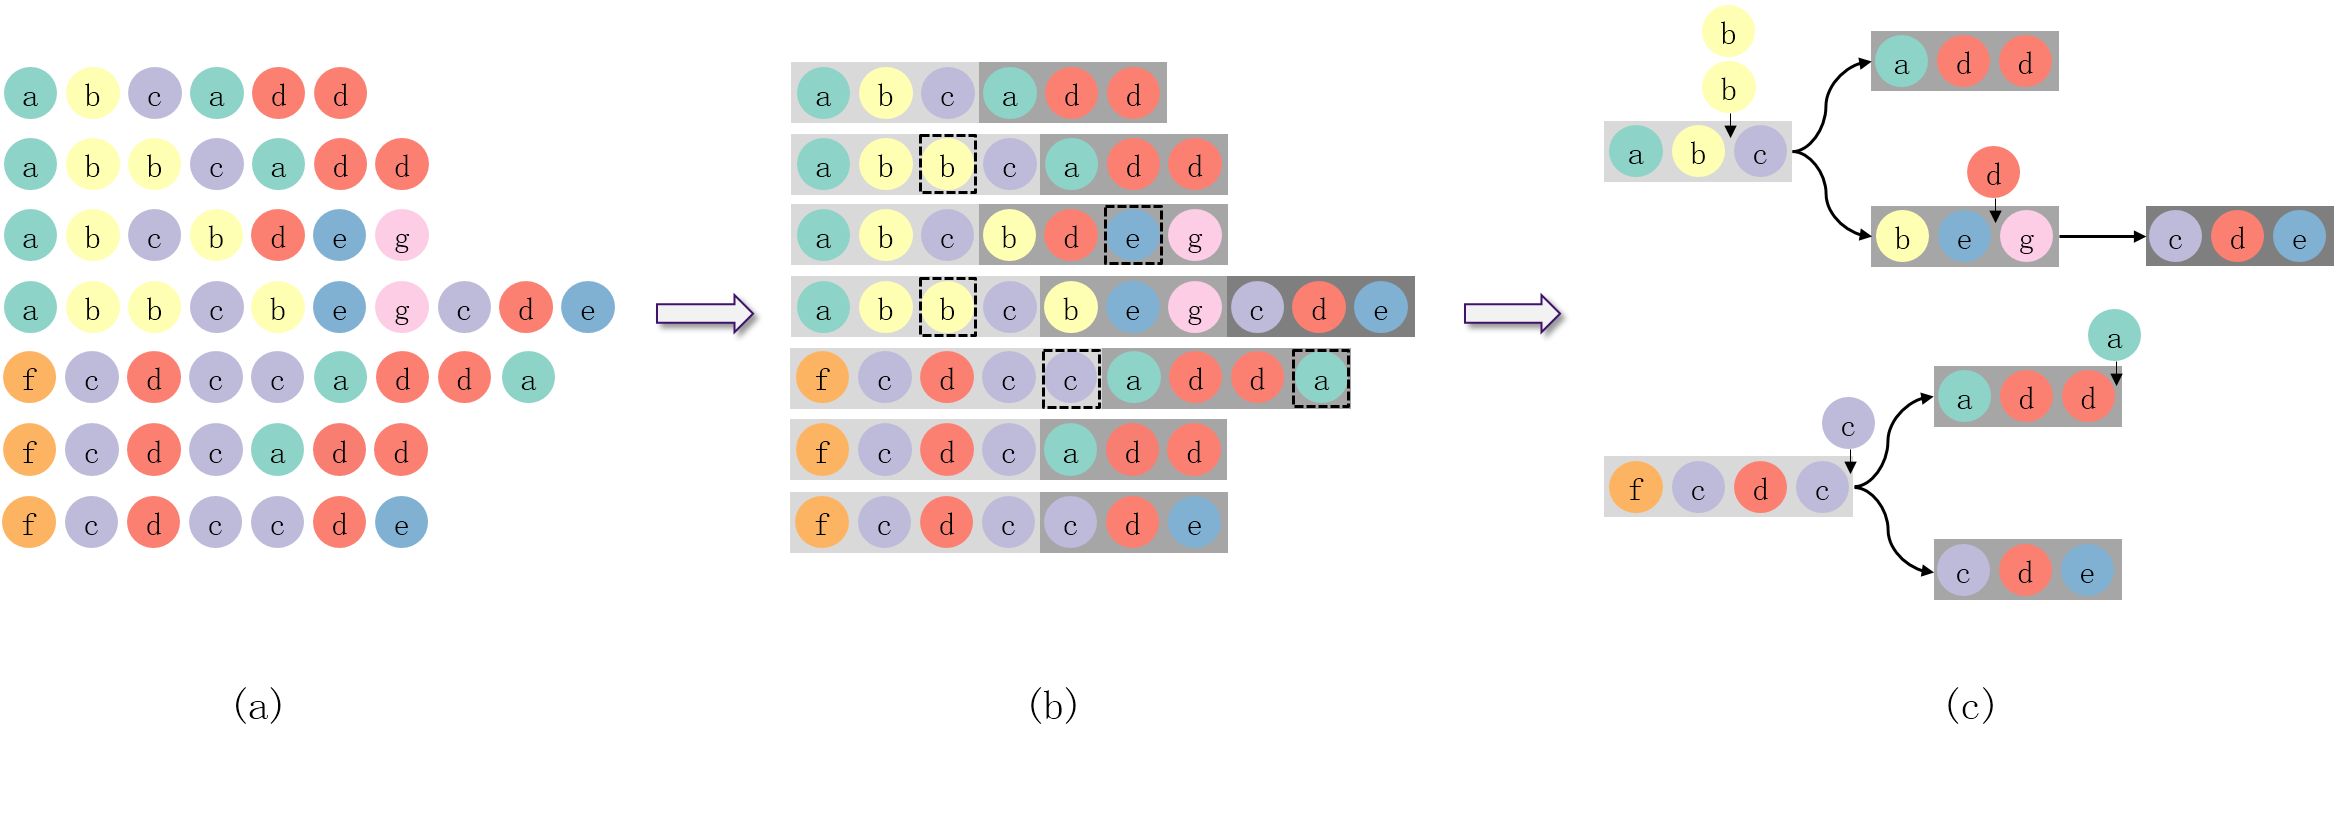
\includegraphics[width=\linewidth]{pictures/summary}
	\caption{stage progression summary 
	}
	\label{fig:summary}
\end{figure*}

\subsection{Sequence Stage Analysis}

A variety of data mining methods have been proposed to identify stages and their progression while few visualization techniques have been studied. Many of the data mining methods focus on the application domains such as medical data analysis. For example, Zhou et al.~\cite{zhou2013modeling} use fused lasso formulation for stage detection. Jackson et al.~\cite{jackson2003multistate} and Wang et al.~\cite{lu2016exploring} both detect the underlying stages based on the Hidden Markov Model. Yang et al.~\cite{yang2014finding} use the EM algorithm to associate stages with sequences. Recently, EventThread~\cite{guo2018eventthread} visualizes the stage progression patterns with storyline visualization. To the best of our knowledge, it is the first work that focuses on stage progression visualization. The main difference between EventThread and StageMap is that EventThread mainly focuses on visual representation and simply extracts stages by uniformly segmenting sequences, while StageMap tries to extract the optimized stages and visually represent the data consistently. 

